\subsection{Meta-learning Representation Learning}
\label{sec:mlr}
Here we propose a model-agnostic meta-learning framework composed of two modules: $\phi_\theta(X)$, a deep Representation Module (RM) parametrized by $\theta$ - from $X$ to $\mathbb{R} ^ {h}$; $g_W$, an Adaption Module (AM) parameterized by $W$ - from $\mathbb{R} ^ {h}$ to $y$. The architecture of this composed module, $f_{\theta, w} = g_W(\phi_\theta(X))$ is shown in figure \ref{img:1} . We follow a similar setup as **: $\theta$ is a meta-parameter that is learned by minimizing the meta-objective and is only updated during meta-training. Then, $W$ is learned from trajectory using fully online stream data in a single pass.

\begin{figure*}[ht]
\centering
    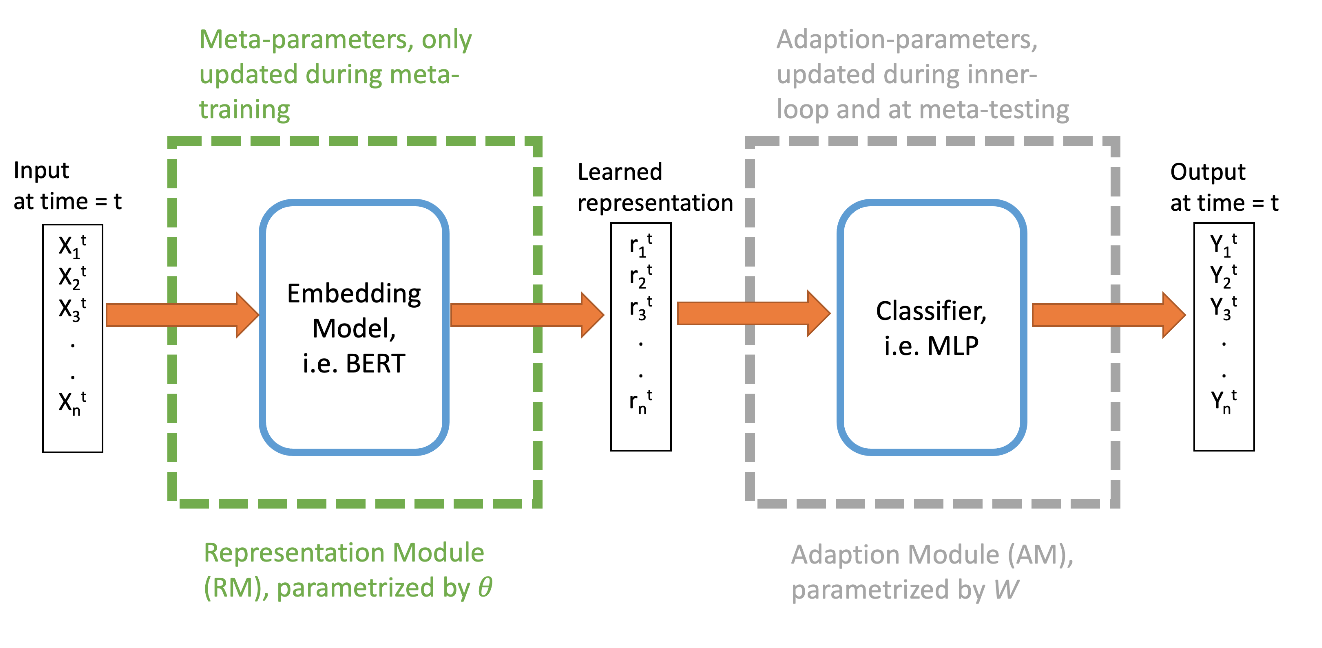
\includegraphics[scale=0.6]{imgs/framework.jpg}
    \caption{Our proposed framework composed of two modules: Representation Module and Adaption Module}
    \label{img:1}
\end{figure*}

We adapted Online-aware Meta-learning (OML) as our meta-objective for updating $\theta$ in Representation Module. OML objective could help maximize fast adaption for training the Representation Module as well as minimizing interference and is defined as:
\begin{equation}
    \begin{aligned}
       \min_{W, \theta} \sum_{\mathcal{T}_i \sim p(\mathcal{T})} \mathrm{OML}(W, \theta) \\
       = \sum_{\mathcal{T}_i \sim p(\mathcal{T})} \sum_{\mathcal{S}_k ^ j \sim p(\mathcal{S}_k | \mathcal{T}_i)} [\mathcal{L}_i (U(W, \theta, \mathcal{S}_k ^ j)]
   \end{aligned}
\end{equation}

where $p(\mathcal{T})$ is the assumed distribution for this continual learning problem; $\mathcal{S}_k ^ j = (X_{j+1}^i, Y_{j+1}^i), ..., (X_{j+k}^i, Y_{j+k}^i)$, a random trajectory of length $k$ sampled from $p(\mathcal{T})$. And $U(W, \theta, \mathcal{S}_k ^ j) = (W_{t+k}, \theta)$ is an updated function where $W_{t+k}$ is the weights of Adaption Module after $k$ steps of parameter updates, where the $jth$ update step in $U$ is on parameters $(W_{t+j-1}, \theta)$ with samples $(X_{j+t}^i, Y_{j+t}^i)$. We can see that OML only uses one data point from the trajectory, $\mathcal{S}_k ^ j$, which would help the model overcome the common problems of catastrophic forgetting in continual learning. 

Here, we use BERT * as our Representation Module due to its strong linguistic representation learning ability and a one-layer fully-connected network as our Adaption Module. 

\subsection{Meta-Training and Meta-Testing Workflow}
As stated in section \ref{sec:mlr}, we update both Representation Module and Adaption Module only in meta-training phase, which is composed of four steps as shown in figure 2 below: 
1. Suppose there is a data stream $\mathcal{T} = (X_0, Y_0), (X_1, Y_1), (X_2, Y_2), ..., (X_n, Y_n)$, we randomly sample a trajectory $\mathcal{S}_{support}$ of length $k$ as our support set for inner updates and another trajectory $\mathcal{S}_{query}$ for evaluation. \\
2. We use $\mathcal{S}_{support}$ to do $k$ continual gradient updates on Adaption Module following OML training objective, from  $W_1$ to $W_2$, ..., to $W_k$. \\
3. Next, we run evaluation of $\mathcal{S}_{query}$ using the updated network to obtain a loss; this loss would be back-propagated with respect to the initial parameters, $\theta$ of RM and $W_1$ of AM. \\
4. Finally we update both of RM and AM, from  $\theta$, $W_1$ to $\theta'$, $W_1'$.

For meta-testing, we would freeze Representation Module and simply update the Adaption Module following the step 2 in meta-training using the support set and then make predictions on query set with the updated Adaption Module and freeze Representation Module.
\begin{figure*}[ht]
\centering
    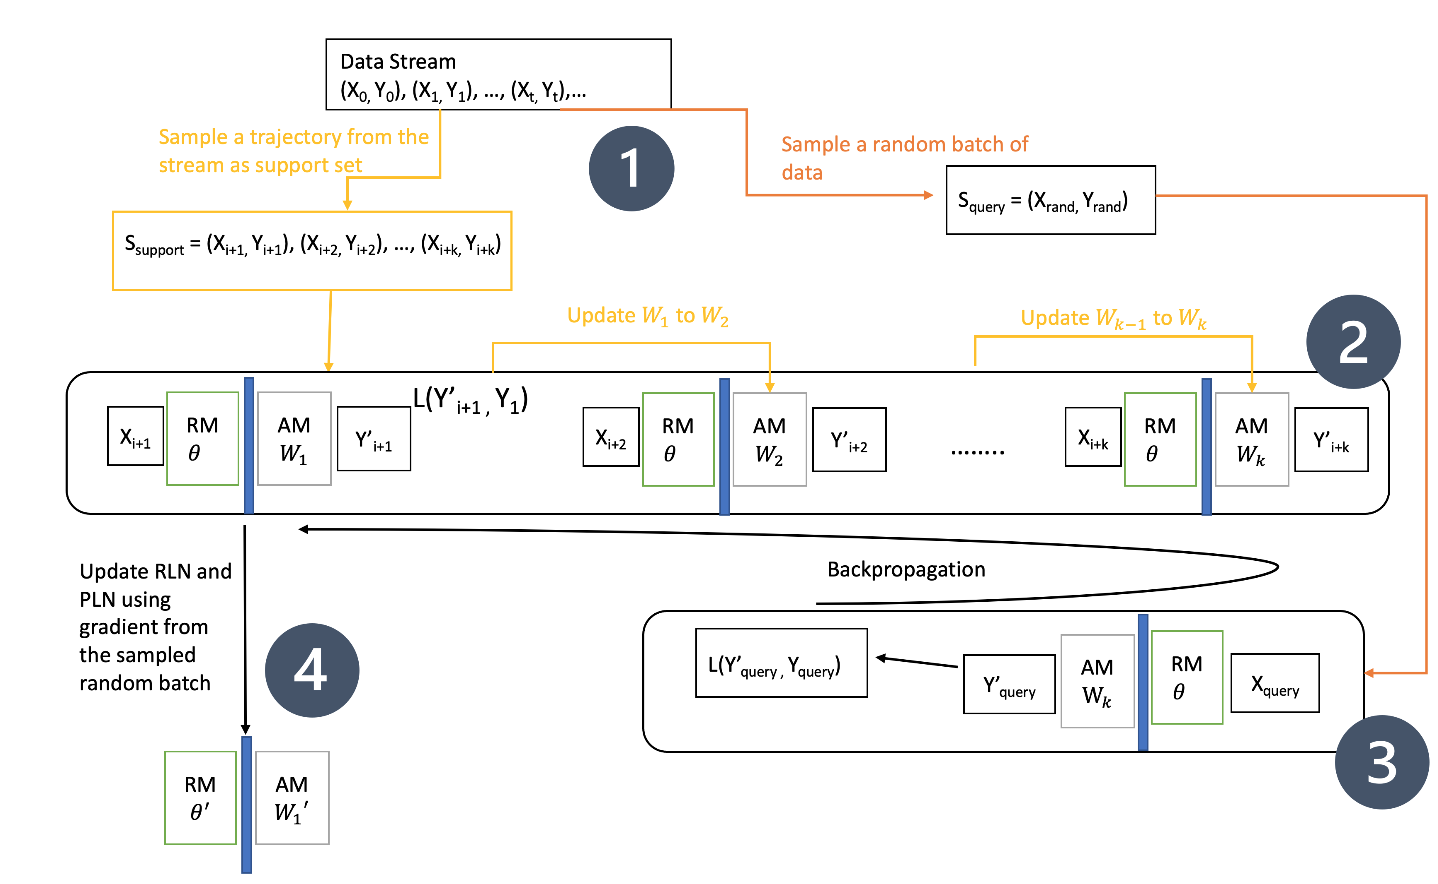
\includegraphics[scale=0.6]{imgs/meta-training.png}
    \caption{Meta-training Workflow}
    \label{img:2}
\end{figure*}
